I've been continuing my efforts to try to break down DALL-E. Bing Image
Creator uses DALL-E and has rapidly increased the quality of its output.
I've been finding that the more complicated the prompt I throw at it the
worse the output looks. Let's look at some examples.

We start with the prompt: ``A female fitness enthusiast visiting her
college's computer lab''

\begin{figure}
\centering
\pandocbounded{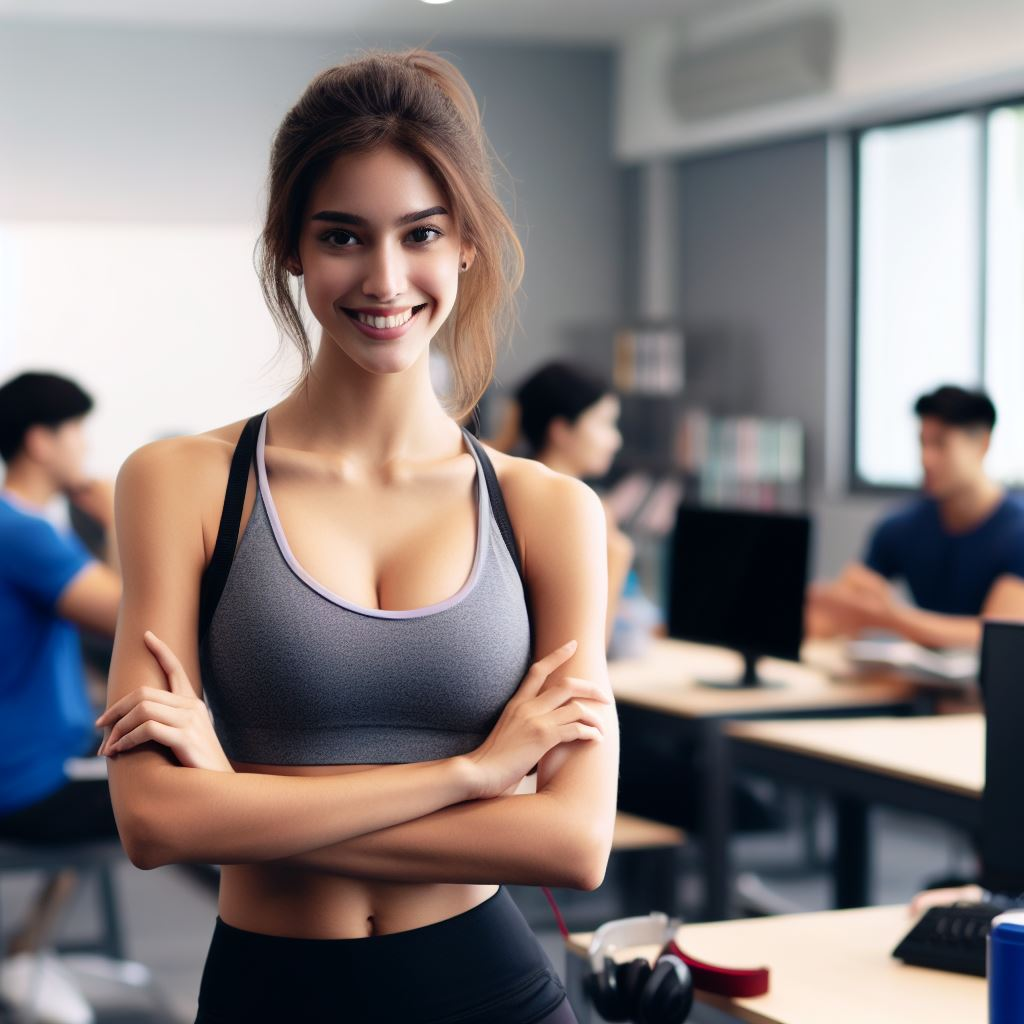
\includegraphics[keepaspectratio]{\%7B\%7Bsite.url\%7D\%7D/img/enthusiast-lab.jpg}}
\caption{Picture generated by the prompt ``A female fitness enthusiast
visiting her college's computer lab''}
\end{figure}

Okay, that's fairly reasonable. Now we can start messing with
complexity. Let's change the prompt to this: ``A female fitness
enthusiast visiting her university's computer lab''

\begin{figure}
\centering
\pandocbounded{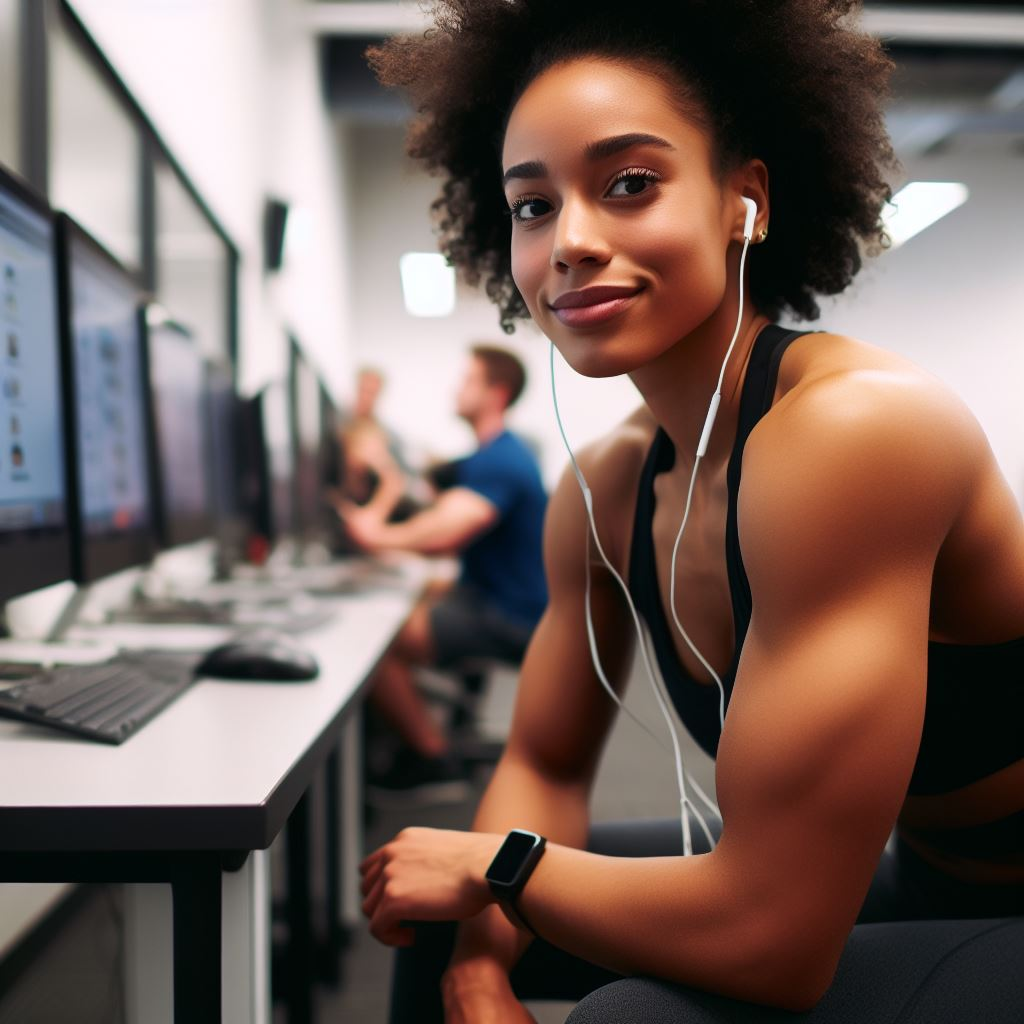
\includegraphics[keepaspectratio]{\%7B\%7Bsite.url\%7D\%7D/img/enthusiast-lab-u.jpg}}
\caption{Picture generated by the prompt ``A female fitness enthusiast
visiting her university's computer lab''}
\end{figure}

Okay, still doing okay. Now to start getting weird. We try this prompt:
``A female soccer enthusiast visiting her university's computer lab''

\begin{figure}
\centering
\pandocbounded{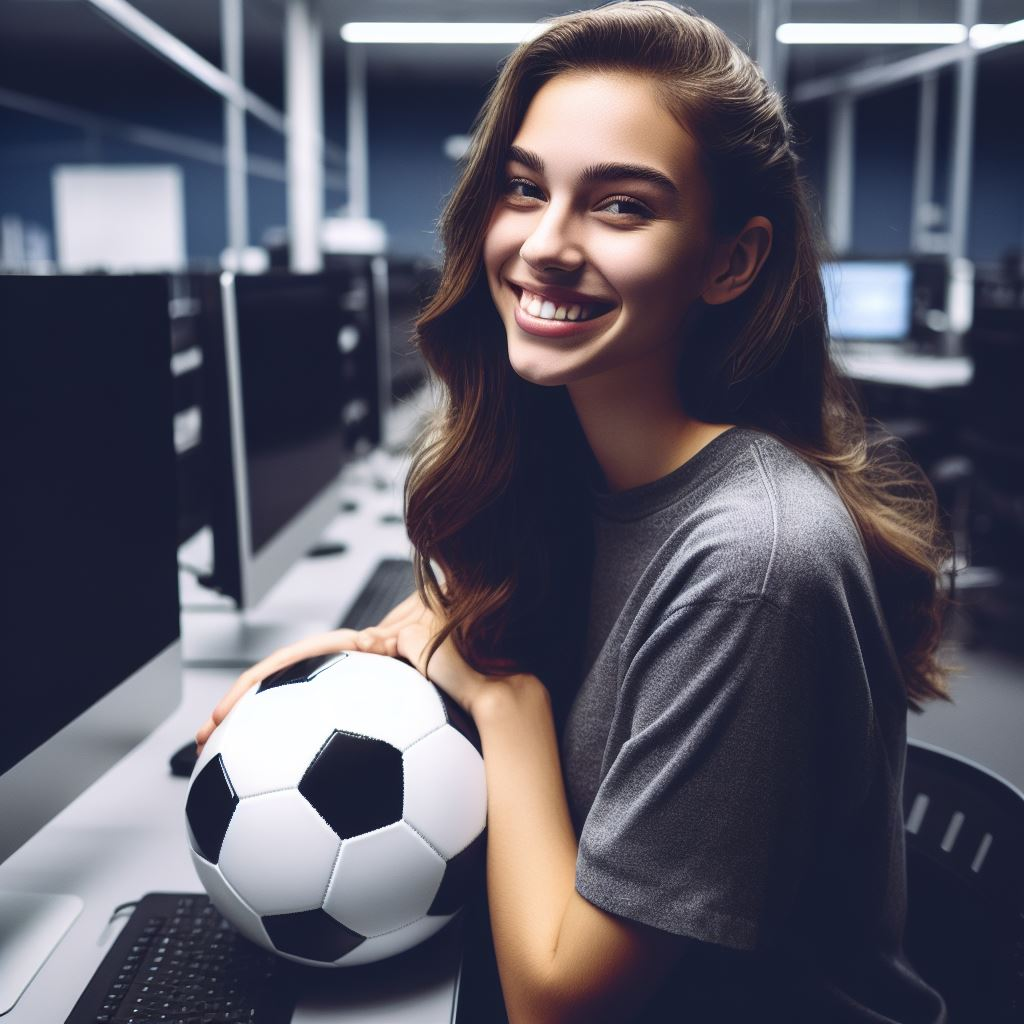
\includegraphics[keepaspectratio]{\%7B\%7Bsite.url\%7D\%7D/img/enthusiast-lab-u-soccer.jpg}}
\caption{Picture generated by the prompt ``A female soccer enthusiast
visiting her university's computer lab''}
\end{figure}

Well, not too weird. Let's try
\href{https://en.wikipedia.org/w/index.php?title=Calvin_and_Hobbes&oldid=1179496024\#Calvinball}{Calvinball}.
That's not real. It was made up by a cartoonist down in Chagrin Falls.
What will the AI do?

\begin{figure}
\centering
\pandocbounded{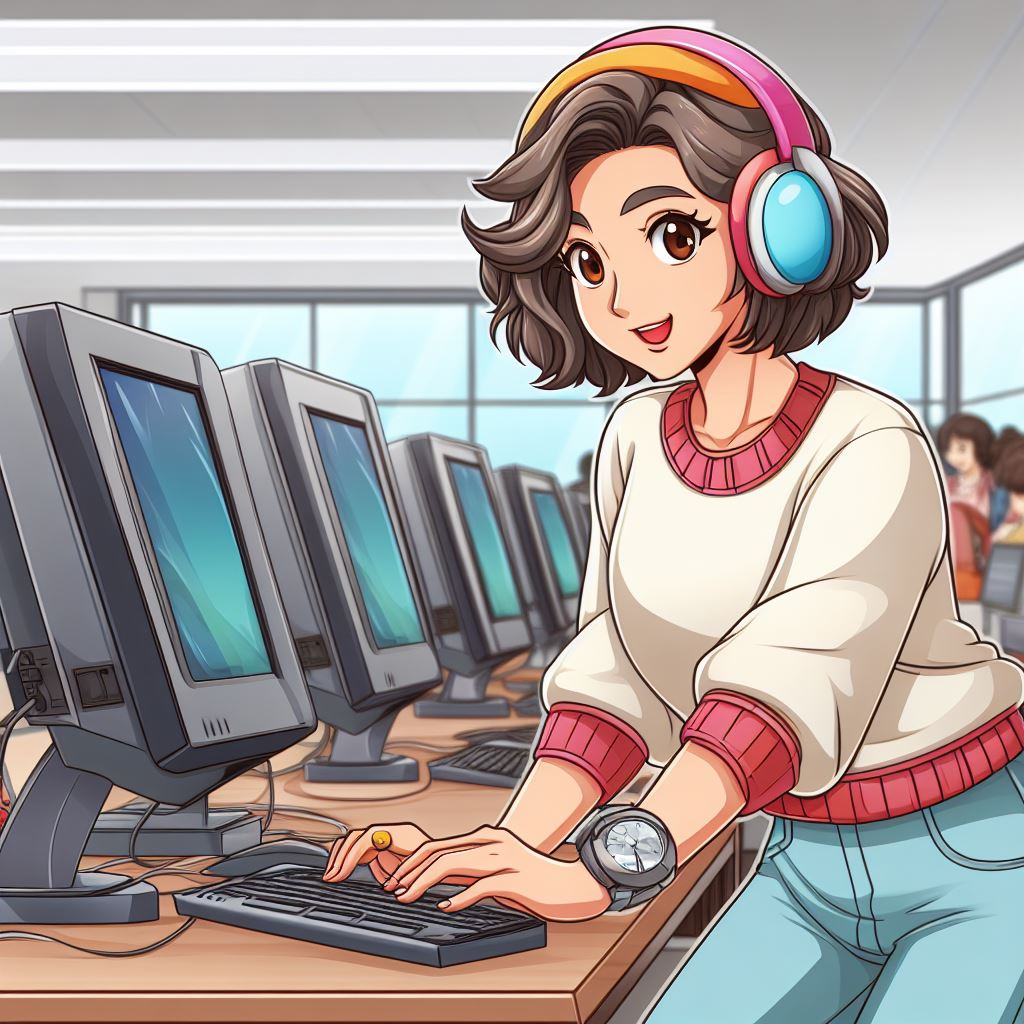
\includegraphics[keepaspectratio]{\%7B\%7Bsite.url\%7D\%7D/img/calvinball-ai.jpg}}
\caption{Picture generated by the prompt ``A female calvinball
enthusiast visiting her university's computer lab''}
\end{figure}

\begin{quote}
\emph{A female calvinball enthusiast visiting her university's computer
lab}
\end{quote}

Well, that definitely looks cartoonish. How about we bring it back
towards reality with mintonette?

\begin{figure}
\centering
\pandocbounded{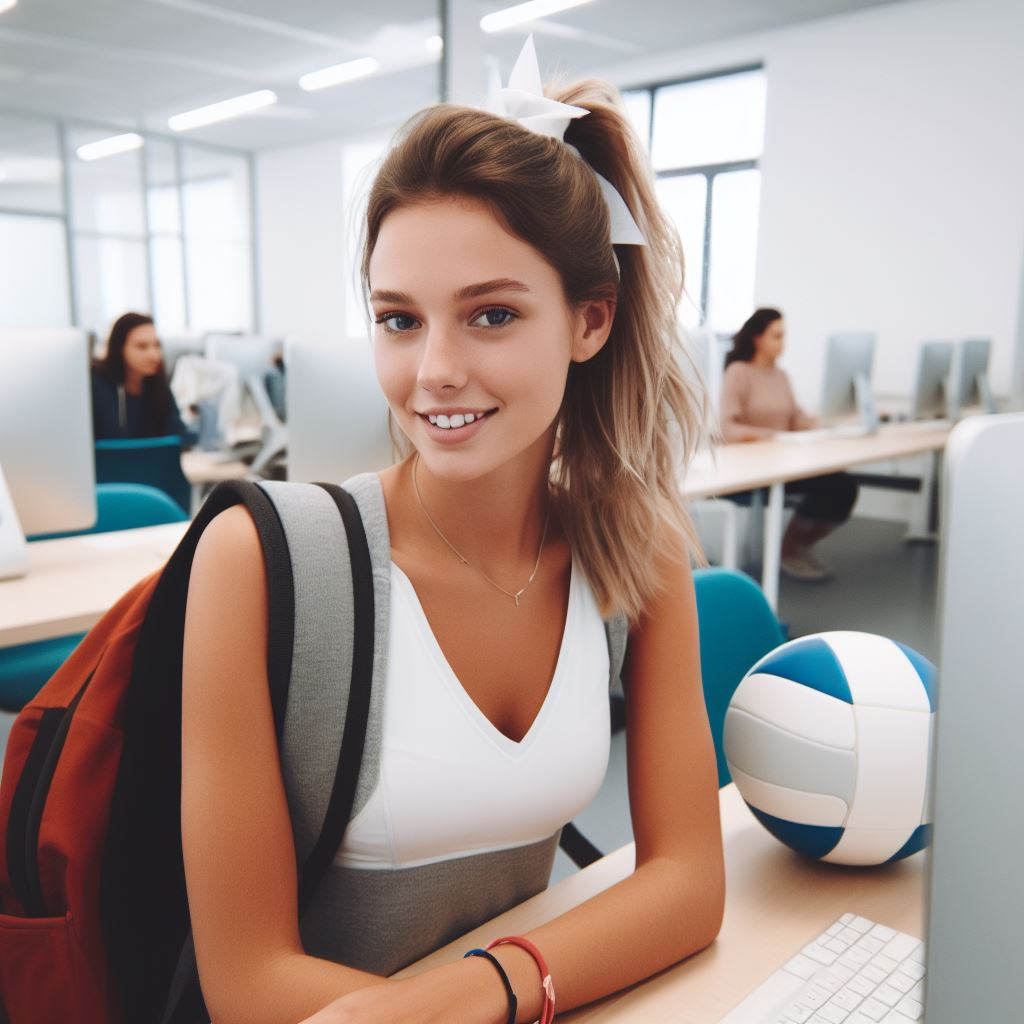
\includegraphics[keepaspectratio]{\%7B\%7Bsite.url\%7D\%7D/img/volleyball-ai.jpg}}
\caption{Picture generated by the prompt ``A female beach volleyball
enthusiast visiting her university's computer lab''}
\end{figure}

\begin{quote}
\emph{A female beach volleyball enthusiast visiting her university's
computer lab}
\end{quote}

Okay, still within the realm of reason. Let's try fantasy then!

\begin{figure}
\centering
\pandocbounded{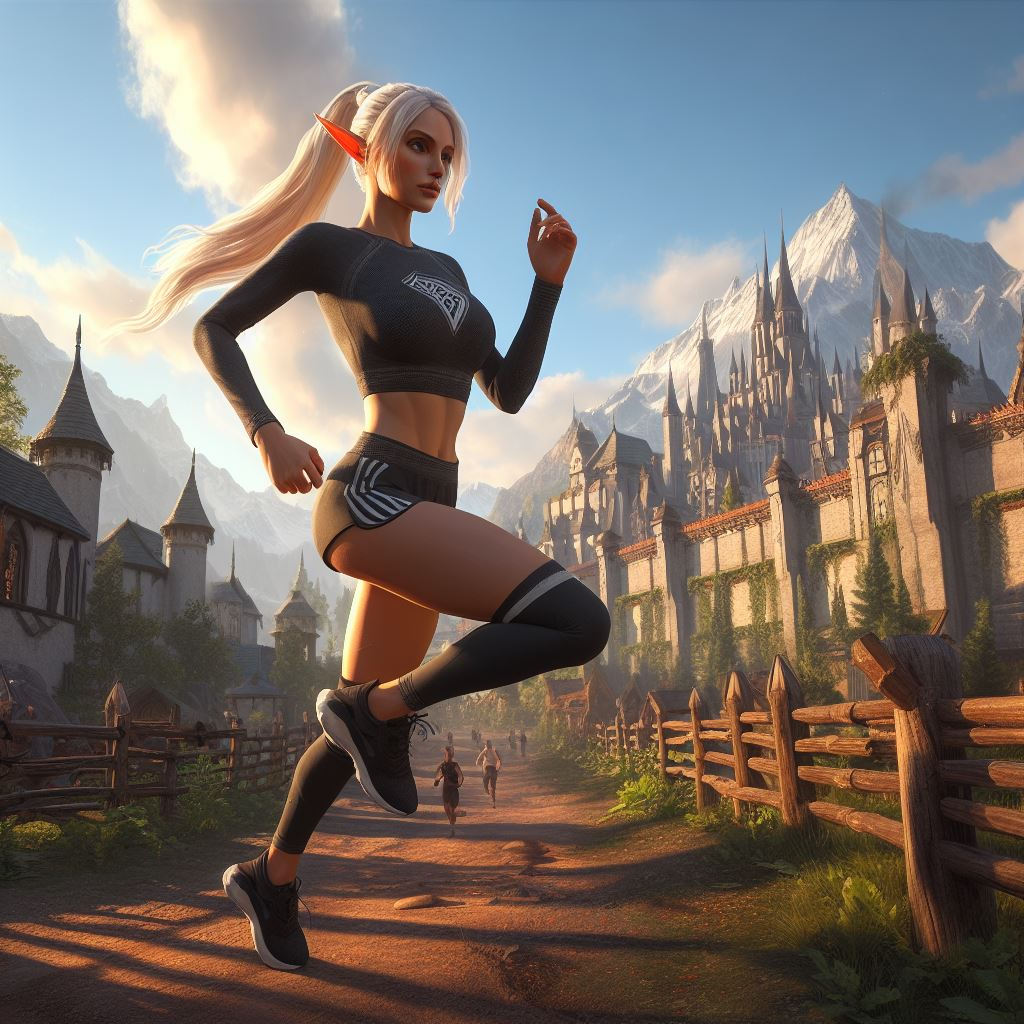
\includegraphics[keepaspectratio]{\%7B\%7Bsite.url\%7D\%7D/img/poached-videogame-graphics-perhaps.jpg}}
\caption{Picture generated by the prompt ``tall lanky half-elf female
fitness enthusiast with a day job as a cleric in Wildemount who is
running an obstacle course''}
\end{figure}

\begin{quote}
\emph{tall lanky half-elf female fitness enthusiast with a day job as a
cleric in Wildemount who is running an obstacle course}
\end{quote}

It almost looks like video game assets that got ripped off or even
stolen there.

Once you start adding complexity in the realm of fantasy the outputs
starting getting weirder. Trying the prompt ``A half-dwarf female
fitness enthusiast from Wildemount who has day jobs as both a cleric for
The Changebringer and as a bard'' gives you this:

\begin{figure}
\centering
\pandocbounded{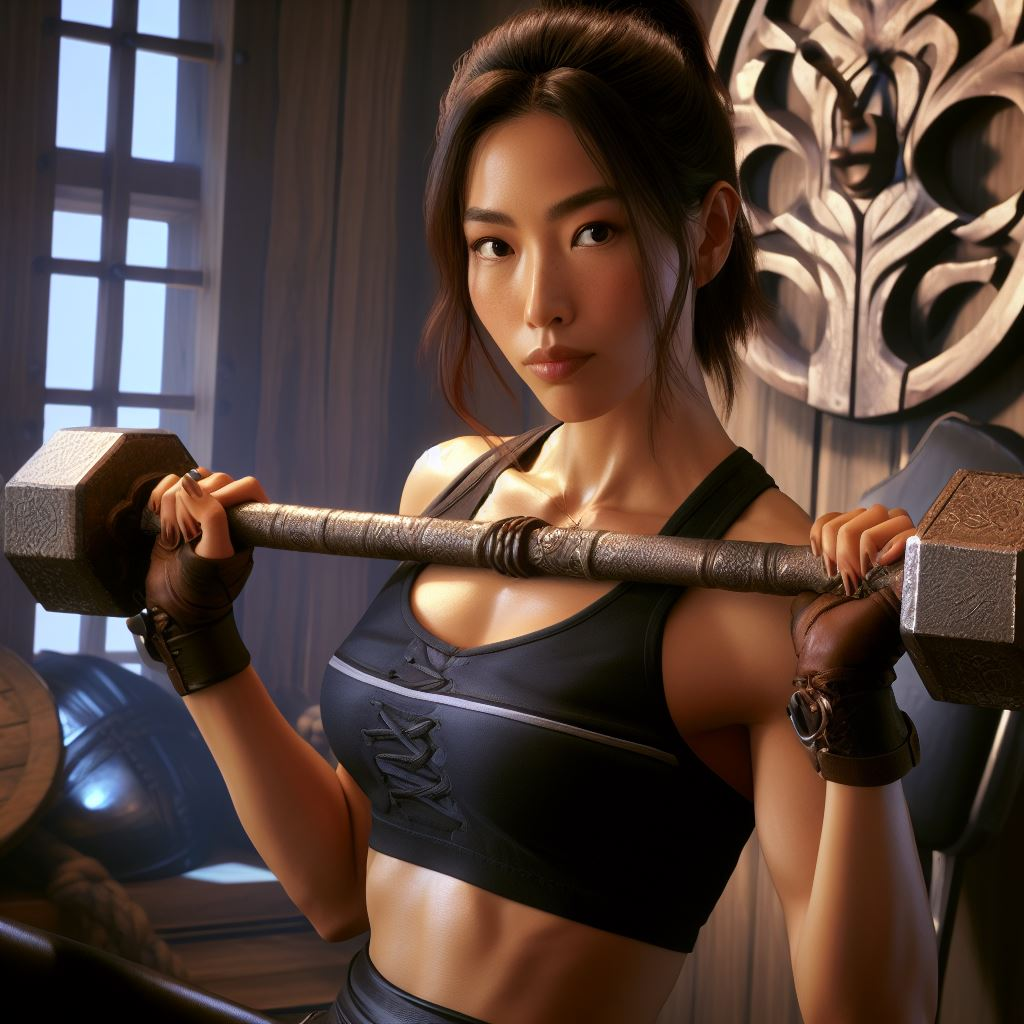
\includegraphics[keepaspectratio]{\%7B\%7Bsite.url\%7D\%7D/img/curling-bard.jpg}}
\caption{Picture generated by the prompt ``A half-dwarf female fitness
enthusiast from Wildemount who has day jobs as both a cleric for The
Changebringer and as a bard''}
\end{figure}

Or then you try ``A half-dwarf female fitness enthusiast from Wildemount
who has a day job as a cleric for both The Changebringer and The
Traveler'' and get this:

\begin{figure}
\centering
\pandocbounded{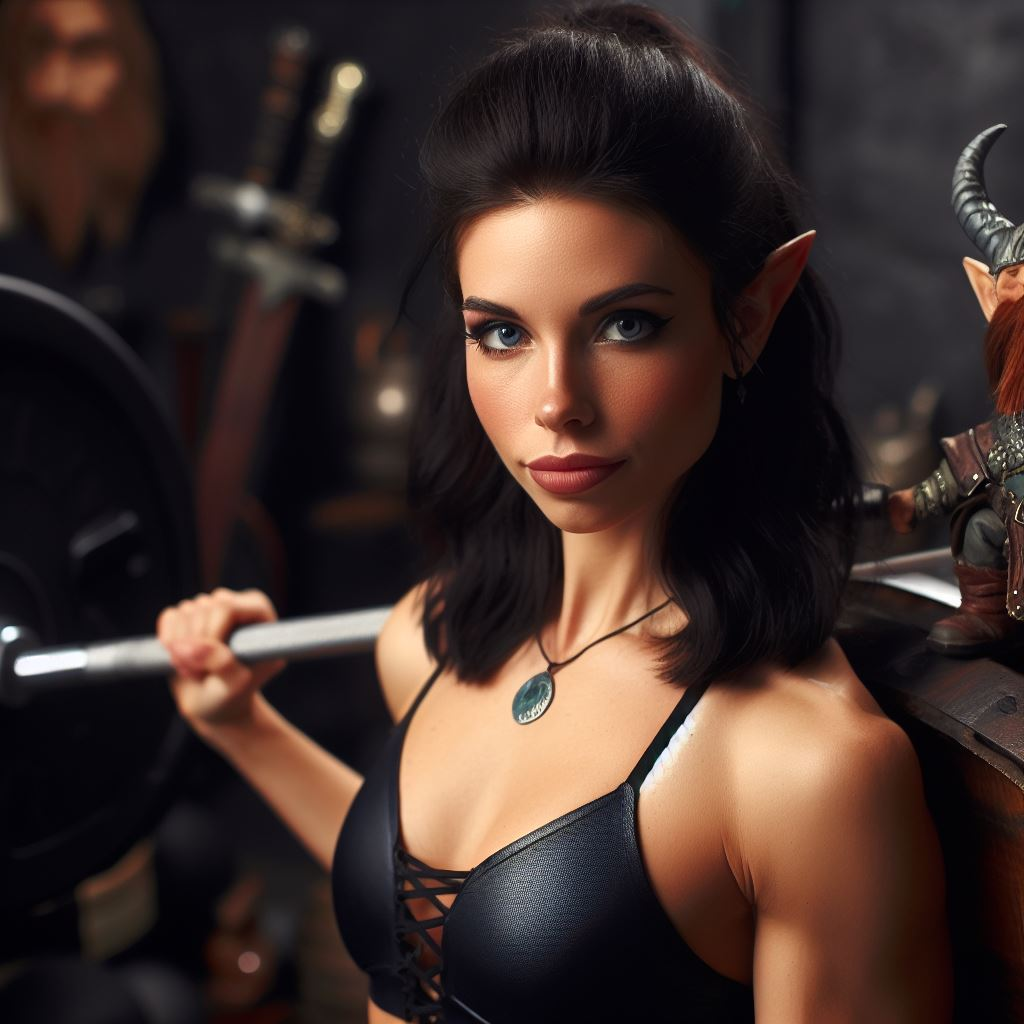
\includegraphics[keepaspectratio]{\%7B\%7Bsite.url\%7D\%7D/img/changebringing.jpg}}
\caption{Picture generated by the prompt ``A half-dwarf female fitness
enthusiast from Wildemount who has a day job as a cleric for both The
Changebringer and The Traveler''}
\end{figure}

Yet a prompt of ``A half-dwarf female fitness enthusiast from Wildemount
who has a day job as a cleric for both The Changebringer and The Dawn
Father'' brings you something like this:

\begin{figure}
\centering
\pandocbounded{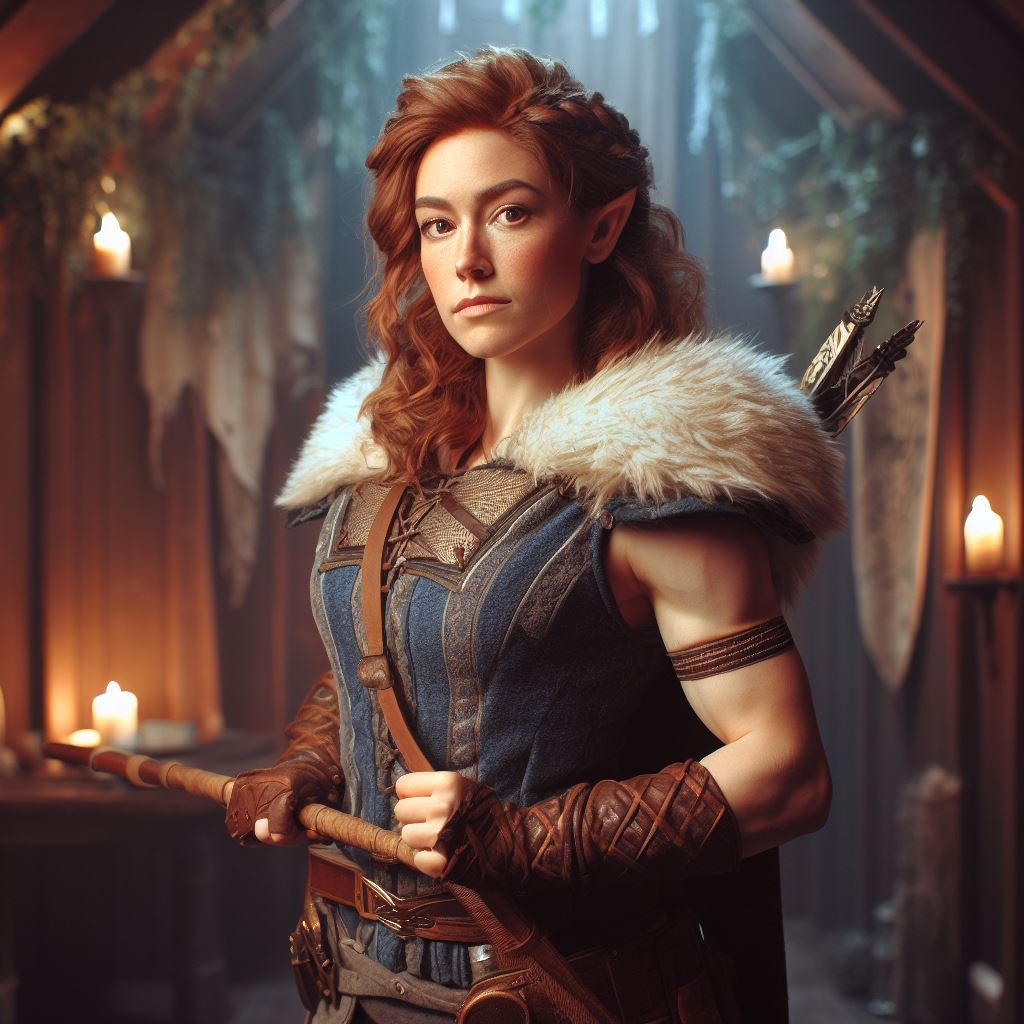
\includegraphics[keepaspectratio]{\%7B\%7Bsite.url\%7D\%7D/img/dawnfather.jpg}}
\caption{Picture generated by the prompt ``A half-dwarf female fitness
enthusiast from Wildemount who has a day job as a cleric for both The
Changebringer and The Dawn Father''}
\end{figure}

In another prompt you start to see the
\href{https://knowyourmeme.com/memes/sarm-goblin}{SARMS Goblin} show up.
The prompt is: ``A half-dwarf female fitness enthusiast from Wildemount
who has a day job as a cleric for The Changebringer who is visiting a
friendly human witch who is also a very tall female fitness
enthusiast.''

\begin{figure}
\centering
\pandocbounded{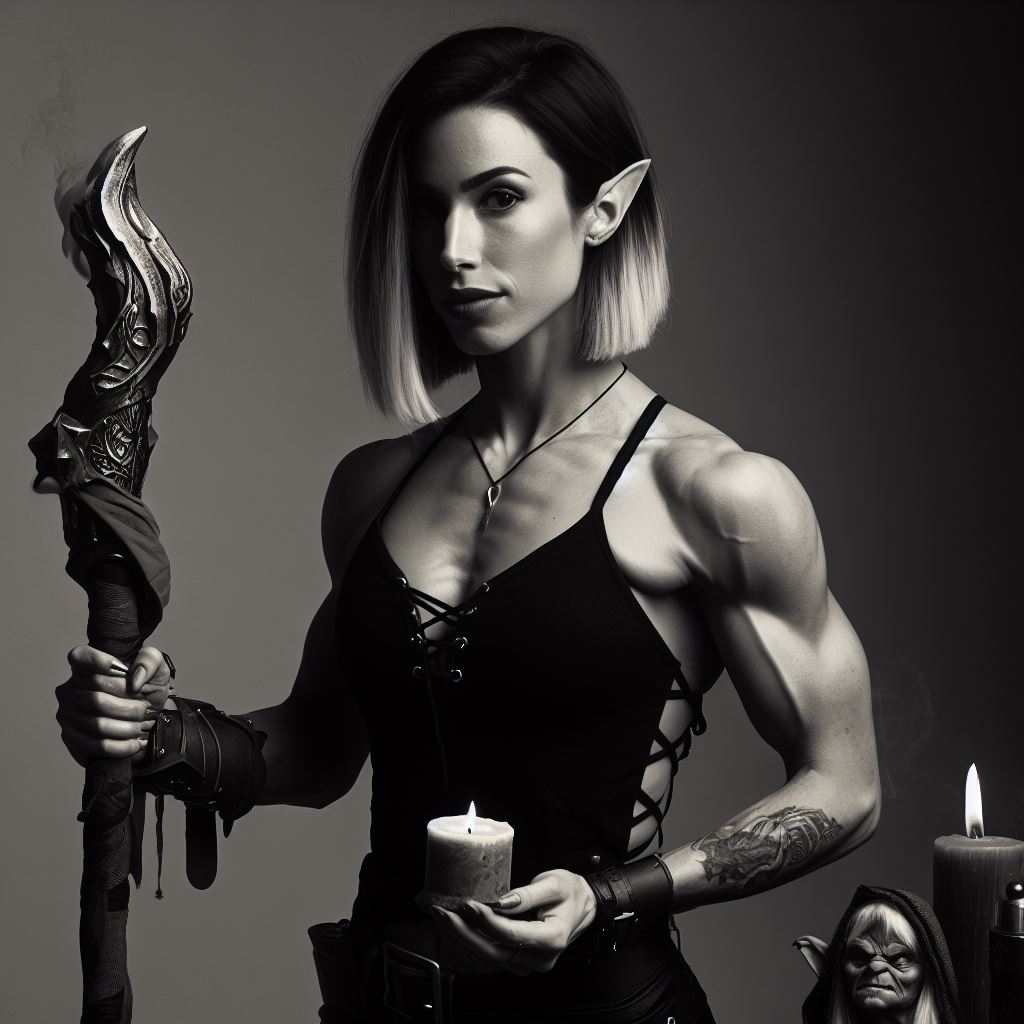
\includegraphics[keepaspectratio]{\%7B\%7Bsite.url\%7D\%7D/img/walkingstick.jpg}}
\caption{Picture generated by the prompt ``A half-dwarf female fitness
enthusiast from Wildemount who has a day job as a cleric for The
Changebringer who is visiting a friendly human witch who is also a very
tall female fitness enthusiast.''}
\end{figure}

The outputs on this prompt were certainly strange: ``A half-dwarf female
fitness enthusiast from Wildemount who has a day job as a cleric for The
Changebringer who is visiting a friendly female fitness enthusiast at
the academy of magic.''

\begin{figure}
\centering
\pandocbounded{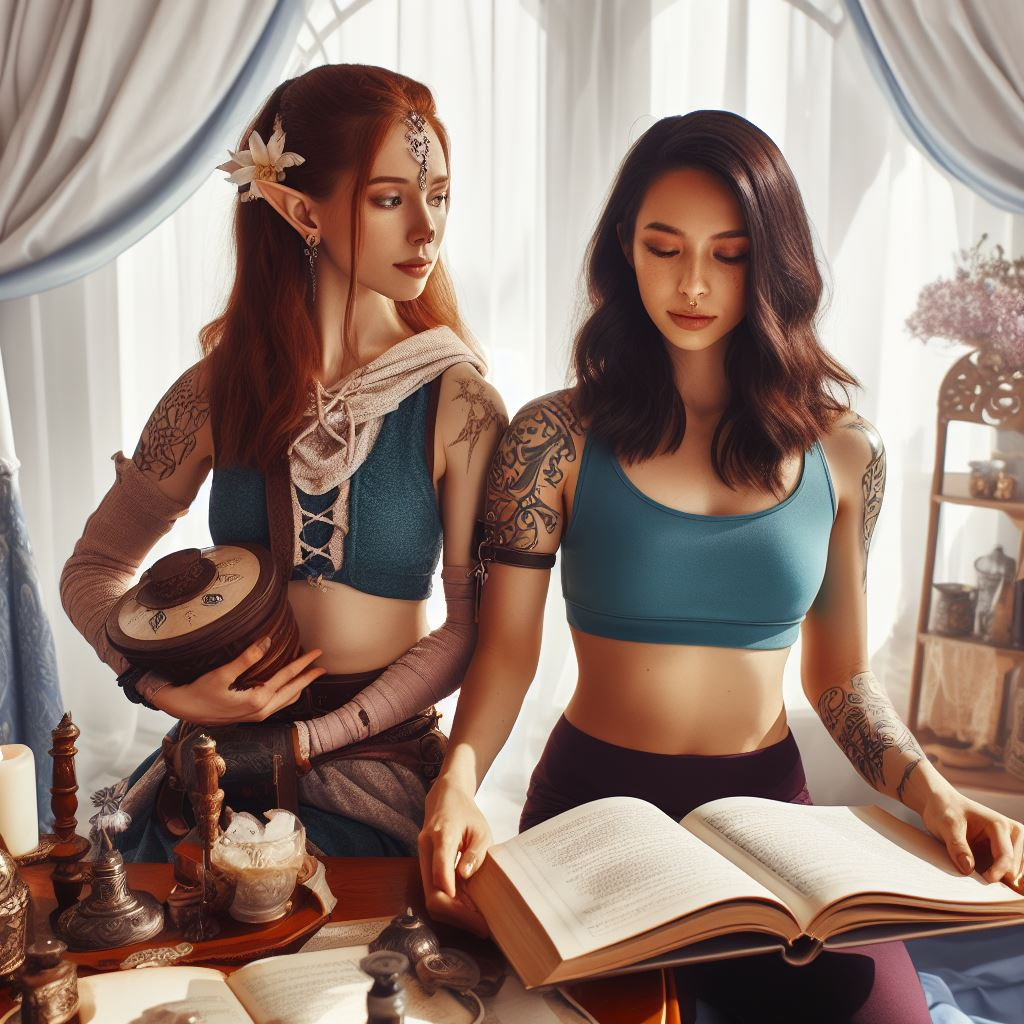
\includegraphics[keepaspectratio]{\%7B\%7Bsite.url\%7D\%7D/img/magicschool.jpg}}
\caption{Picture generated by the prompt ``A half-dwarf female fitness
enthusiast from Wildemount who has a day job as a cleric for The
Changebringer who is visiting a friendly female fitness enthusiast at
the academy of magic.''}
\end{figure}

Starting with a simple prompt and making it increasingly absurd didn't
work in terms of breaking things. Back to the drawing board, I guess.
Testing the limits of this tech does help when I have to deal with
students asking questions about Generative AI. I can't always just show
them
\href{https://arstechnica.com/information-technology/2023/05/ai-generated-beer-commercial-contains-joyful-monstrosities-goes-viral/}{\emph{Synthetic
Summer}} and say that this tech creates monstrosities. It is constantly
changing and society is really, really not ready for the implications of
what may result.
